\documentclass{article}
\usepackage{amsmath}
\usepackage{graphicx}
\usepackage{hyperref}
\usepackage{subcaption}
\usepackage{cleveref}
\usepackage[margin=1in]{geometry}
\makeatletter
\newcommand\footnoteref[1]{\protected@xdef\@thefnmark{\ref{#1}}\@footnotemark}
\makeatother
\title{PhD Progress}
\author{Marco Cucchi}
\date{\today}
\begin{document}
\maketitle
\tableofcontents
\newpage

\section{Introduction}

This document is a log-book for all the work done during my PhD project.
All code used con be found on github repository \url{https://github.com/marco-cucchi/L96gev}.

\section{EVT and the Lorenz-96 model}

Aim of this work is to find EVT parameters for observables of the Lorenz-96 (L96) model, and compare them with the bounds provided in \cite{LucariniExtremesBook}.

\subsection{Lorenz-96 model simulations} \label{gev_sim}

As a first step, a number of independent simulations of the L96 model are performed.
The L96 model is defined as follows. For $i=1,...,N$:

\begin{equation}
\frac{dx_i}{dt} = (x_{i+1}-x_{i-2})x_{i-1} - x_i + F
\end{equation}

where it is assumed that $x_{-1}=x_{N-1}$, $x_0 = x_N$ and $x_{N+1}=x_1$. Here $x_i$ is the state of the system on the $i$-th coordinate, and $F$ is the forcing constant.
For this set of simulations, values of $F$ and $N$ have been set to $F=8$ and $N=32$.\\
Integration has been conducted using 4-\textit{th} order Runge-Kutta scheme, with integration step $dt=10^{-2}$. Initial conditions for each simulation have been set equal to

\begin{equation}
x_i^0 = 8 + \epsilon, \quad \epsilon \sim U([-0.05,+0.05])
\end{equation}

Different levels of spatial aggregation, defined as $A=32,16,8,4,2,1$, have been considered:

\begin{itemize}
	\item For $A=32$ no aggregation is performed, and each value $x_i$ is treated independently;
	\item For $A=1$ all original $N$ $x_i$ values are spatially averaged into one single value $\overline{x}$ for each time-step;
	\item More in general, for $A=K$ the $N$ spatial coordinates indicated by the index $i$ are divided into $K$ non-overlapping clusters $c_j$ fixed in time, and corresponding $x_i$ values belonging to the same cluster are averaged at each time-step.
\end{itemize}

As observable, the local energy of the system for different levels af aggregation

\begin{equation}
E_j=\frac{1}{2}x_j^2, \quad x_j=
	\begin{cases}
   		x_i, & A=32\\
   		\overline{x} = \frac{1}{N} \sum_{i=1}^{N} x_i & A=1 \\
		\frac{1}{\#c_j} \sum_{i \in c_{j, K}} x_i & A=K
	\end{cases}
\end{equation}

is considered.

In order to extract information on the statistics of extremes, very long simulations have to be performed. In order to find a good compromise between this requirement and the limited amount of disk space, a similar procedure to the one adopted in \cite{Galfi} has been followed: instead of keeping all values of each simulation, only block-maxima are retained, with block size $\Delta t = 0.5$. It is important to highlight that block-maxima are computed \textit{after} aggregation (spatial average).

Following this procedure, for each simulation (initial condition) 6 different files are obtained, each corresponding to one particular aggregation level $A$: each of these files, then, contain $A$ time-series of block-maxima, one for each of the $A$ clusters.

Script: \href{https://github.com/marco-cucchi/L96gev/commit/f3614ce9369484bc5d1f06613fbea6fe26a7dd87#diff-bdb8a6ca7f3a8d1a4753b03a3b753204}{c003e11}.

\subsection{Statistics of Extreme Events}
\label{subsec:StatExtrEv}

Parameters defining GEV distribution are estimated using three different approaches:

\begin{itemize}
	\item Direct fit using \textit{block-maxima} approach;
	\item Direct fit using \textit{POT} approach (still not described hear);
	\item Method of \textit{moments} described in \cite{LucariniExtremesBook}.
\end{itemize}
Finally, estimates derived with these approaches are compared among them and with bounds related to attractor's dimensions described in \cite{Galfi}.

\subsubsection{Block-maxima approach}

In this approach, each time-series for each different cluster of each simulation is fitted against GEV family of distribution separately. More specifically, for each cluster time-series belonging to a different simulation the following procedure is carried out:

\begin{enumerate}
	\item Percentiles' orders $p$ of interest are fixed (e.g. 0.99, 0.995, ...), and corresponding percentiles (thresholds) $T_p$ are computed; \footnote{This could be something to think upon; in this way I have (slightly?) different percentiles for different time-series in the same simulation and for different simulations. Is this right? The underlying assumption in this procedure should is that all time-series belonging to all simulations should come from the same distribution. So shouldn't the percentiles be the same for all of them?\label{fn1}}
	\item Time-series is divided in $n$ blocks, where $n=length(\text{time-series})(1-p)$;
	\item Compute maxima for each block;
	\item Fit GEVD family to the block-maxima series.
\end{enumerate}

The fit is performed with the R function \texttt{gevFit} from the package \texttt{fExtremes}, using MLE approach. As a result estimations of shape parameter $\xi$, location parameter $\mu$ and scale parameter $\sigma$ are returned, with respective uncertainties as computed via MLE.\\
Location parameter $\mu$ is actually assigned the value $T_p$; the \textit{absolute maximum} from each time-series is also kept; \textit{modified scale parameter} $\sigma^*$ is computed as

\begin{equation} \label{sigma_mod}
\sigma^*=\sigma-\xi T_p
\end{equation}
Error on $\sigma^*$ is estimated via propagation of error.\\
As explained in \cite{Coles}, in order to find a valid threshold value $T_0$ for excess to follow generalized Pareto distribution (and, consequently, GEV distribution), it is a good practice to plot $\xi$ and $\sigma^*$ against $T_p$ and look for the value where both start to be approximately constant: that value is $T_0$.\\
Once parameters have been estimated for all clusters in a simulation, a single estimation of each parameter is saved as the average among all estimates.\footnote{The \textit{absolute maximum} is also averaged, and this could be an error. The average of the \textit{location parameter} $\mu$ is also a little disturbing, but this could be solved following reasoning in footnote \ref{1}. Error computation should be checked.\label{fn2}}
Furthermore, the following parameters are estimated for each simulation:

\begin{itemize}
	\item \textit{scale parameter} $\sigma$ is computed with inverse of equation \ref{sigma_mod}, and relative error is computed via propagation of errors; \footnote{This sounds very stupid, since $\sigma$ was originally estimated (but not saved) via MLE fit to GEVD.\label{fn3}}
	\item \textit{upper end-point} is computed as\footnote{Find reference}
	\begin{equation}
	\hat{uep}=\hat{\mu}-\frac{\hat{\sigma}}{\hat{\xi}}
	\end{equation}
	and the relative error is computed via propagation of errors.
	
\end{itemize}
Finally, for each different aggregation, ensemble averages of \textit{shape} and \textit{modified scale} among all simulations are computed.

\subsubsection{Method of Moments}

Following theory described in \cite{LucariniExtremesBook}, we want to estimate \textit{shape} and \textit{scale} parameters using the following equations (Par 8.2.6 in \cite{LucariniExtremesBook}):

\begin{equation}
\xi_A^{T} = \frac{1}{2}\left(1-\frac{(\langle\tilde{A}_1^{T}\rangle)^2}{\langle\tilde{A}_0^T\rangle \langle\tilde{A}_2^T\rangle - (\langle\tilde{A}_1^{T}\rangle)^2} \right) \label{shape_mom}
\end{equation}
\begin{equation}
\sigma_A^{T} = \frac{1}{2} \frac{\langle\tilde{A}_1^T\rangle \langle\tilde{A}_2^T\rangle} {\langle\tilde{A}_2^T\rangle \langle\tilde{A}_0^T\rangle - \langle\tilde{A}_1^{T}\rangle^2}
\end{equation}
where $A(x)$ is an observable of the system, $T$ is a threshold value and
\begin{equation}
\langle\tilde{A}_n^T\rangle = \int\mu(dx)\Theta(A(x)-T)(A(x)-T)^n,
\end{equation}
being $\Theta$ the Heaviside distribution. This results are exact in the limit for $T \rightarrow A_{max}$.\\
In order to perform this computation, the following procedure has been adopted. First, for each cluster time-series belonging to a different simulation:
\begin{enumerate}
	\item Percentiles' orders $p$ of interest are fixed, and corresponding percentile (thresholds) $T_p$ are computed (footnote \ref{fn1});
	\item $\langle\tilde{A}_n^{T_p}\rangle$ for $n=0,1,2$ are computed, using temporal average in place of ensemble average (assuming ergodicity).\footnote{No standard deviation has been computed at this stage!}
\end{enumerate}
Once moments have been estimated for all clusters in a simulation, a single estimation of each moment is saved as the average among all estimates, and relative standard deviations are computed.\\
Using these estimates, \textit{shape} parameter is computed through equation \ref{shape_mom} and estimation of uncertainty is computed via propagation of error. Finally, for each different aggregation, ensemble averages among all simulations are computed.

\subsubsection{Bounds to the \textit{shape} parameter from the attractor's dimensions}

We want to verify relation (8.2.15) in \cite{LucariniExtremesBook}, which states that

\begin{equation}
\left(d_s +d_u + d_n\right)/2 \leq \delta \leq d_s + \left(d_u + d_n\right)/2,  
\end{equation}
where
\begin{itemize}
	\item $d_u$ is equal to the number of positive Lyapunov exponents of the system \cite{Ott};
	\item $d_n$ is equal to the number of zero Lyapunov exponents of the system, and in particular it is 1 for Axiom A systems \footnote{We are taking this for true in our system};
	\item $d_s = n + \sum_{k=1}^n \lambda_k / \vert \lambda_{n+1} \vert - d_u - d_n$ \cite{Galfi}, with $\lambda_k$ denoting the Lyapunov exponents of the system, in a descending order, and $n$ is such that $\sum_{k=1}^n \lambda_k$ is positive and $\sum_{k=1}^{n+1} \lambda_k$ is negative;
	\item $\xi = -1/\delta$;
	\item $\sigma = \left( A_{max} - T\right)/\delta$, with $A_{max}$ and $T$ denoting the maximum observed value of the observable\footnote{or the \textit{upper end point}?} and the threshold value.
\end{itemize}

Lyapunov exponents have been computed using Benettin algorithm with QR decomposition. Bounds have been computed and averaged over 50 iterations (simulations).
\\Script:
\begin{itemize}
	\item Lyapunov exponents computation: \href{https://github.com/marco-cucchi/L96gev/commit/136afd42b03778e04fe515e517c3e63c406b2043#diff-2a3c128ef27f1e284787331bae1833ea}{136afd4}
	\item Average bounds computation:
	
\end{itemize}

\subsection{Statistics of Extreme Events: Corrections and Results}

In this section results of the analyses reported in Sec. \ref{subsec:StatExtrEv} are described, after issues highlighted in the footnotes \ref{fn1},\ref{fn2},\ref{fn3}.
\\Script:
\begin{itemize}
	\item quantiles computation: \href{https://github.com/marco-cucchi/L96gev/commit/6880d207820a5b5919b3bbd0a034782f34c7bb49#diff-3b01235fe20ba4105fab7b053c2dadfb}{6880d20}
\end{itemize}

\subsubsection{Block-maxima approach}

The following corrections have been applied:

\begin{itemize}
	\item Percentiles are computed once, concatenating the first 80 simulations of the first clusters for each aggregation;
	\item Shape, scale and location parameters from fit procedures are saved for each cluster in each simulation. Averages and computation of derived parameters come after;	
\end{itemize}
Results are shown in Fig. \ref{fig:shape_mle} and \ref{fig:modscale_mle}.
\\Script:
\begin{itemize}
	\item fit: \href{https://github.com/marco-cucchi/L96gev/commit/240d6d0471ddc3fc53789e43e03a87013d032b86#diff-9576f7ab149830e9a08339b0fc9f2569}{240d6d0}
	\item parameters derivation and plots: \href{https://github.com/marco-cucchi/L96gev/commit/97925ef80db61ade1851bb7c41948d7f13f3b91f#diff-9ecb506d1ae86460add99c76d6c9961a}{97925ef}
\end{itemize}


\begin{figure}
	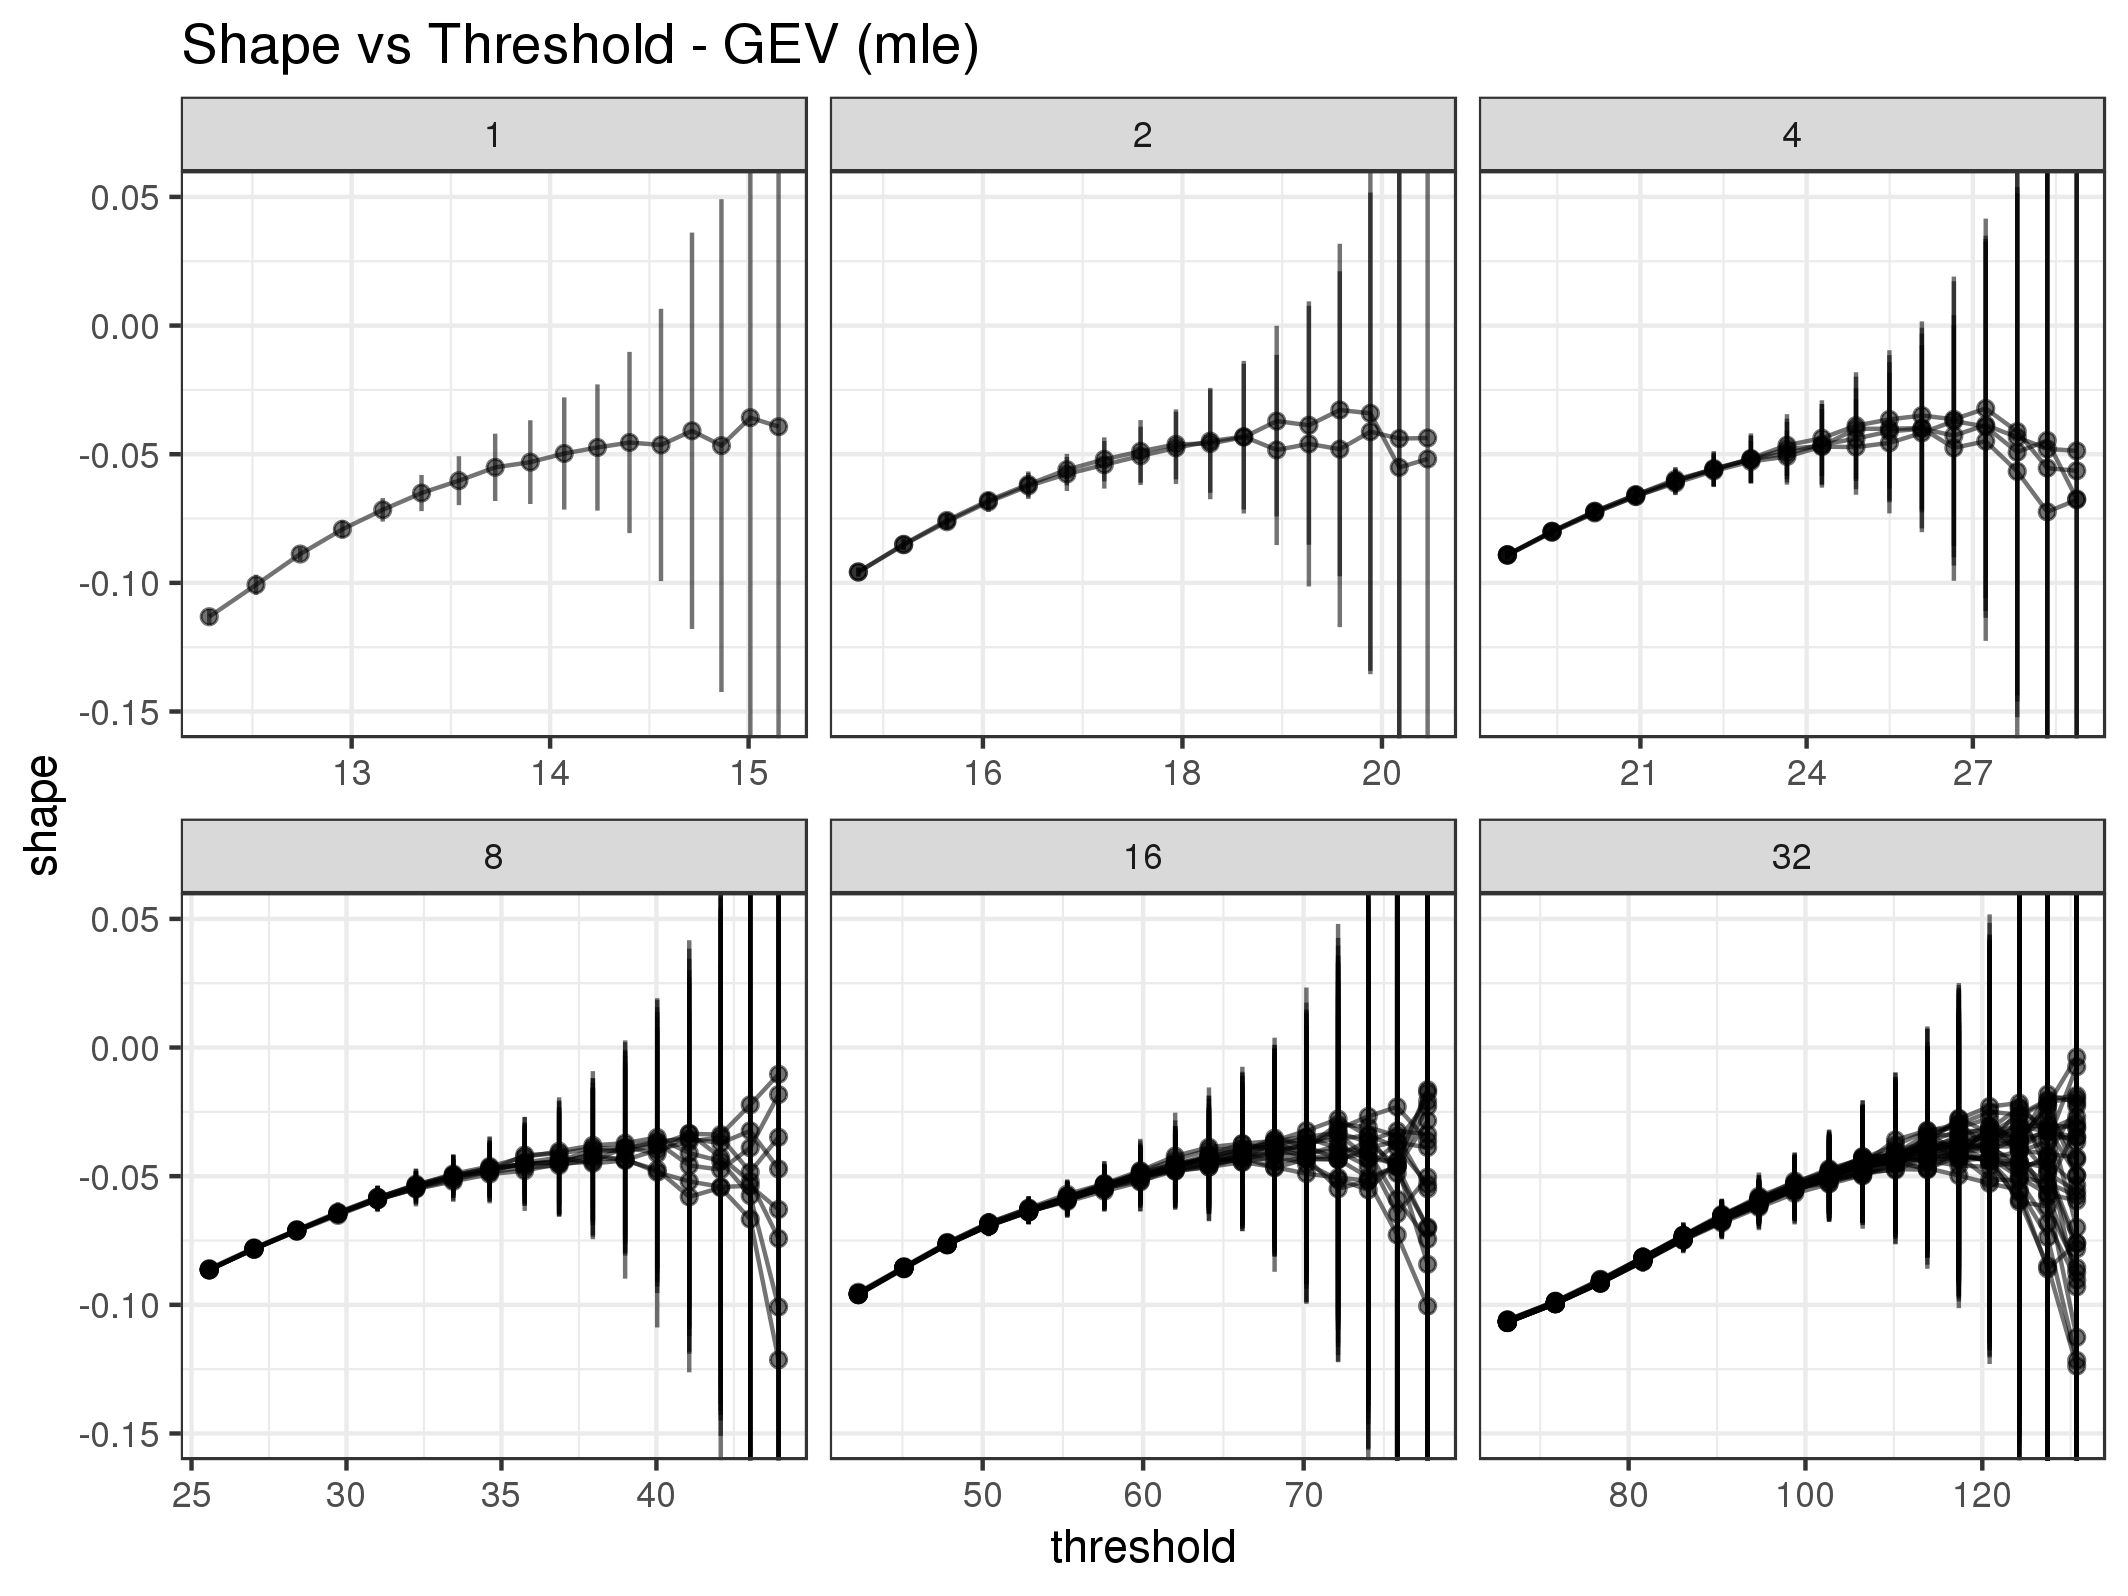
\includegraphics[width=\linewidth]{fig/shape_gev_mle_RK401_1e7_maxt05_1e7.png}
	\caption{Ensemble average of \textit{shape} parameter over 92 simulations. Each cluster is treated separately.}
	\label{fig:shape_mle}
\end{figure}

\begin{figure}
	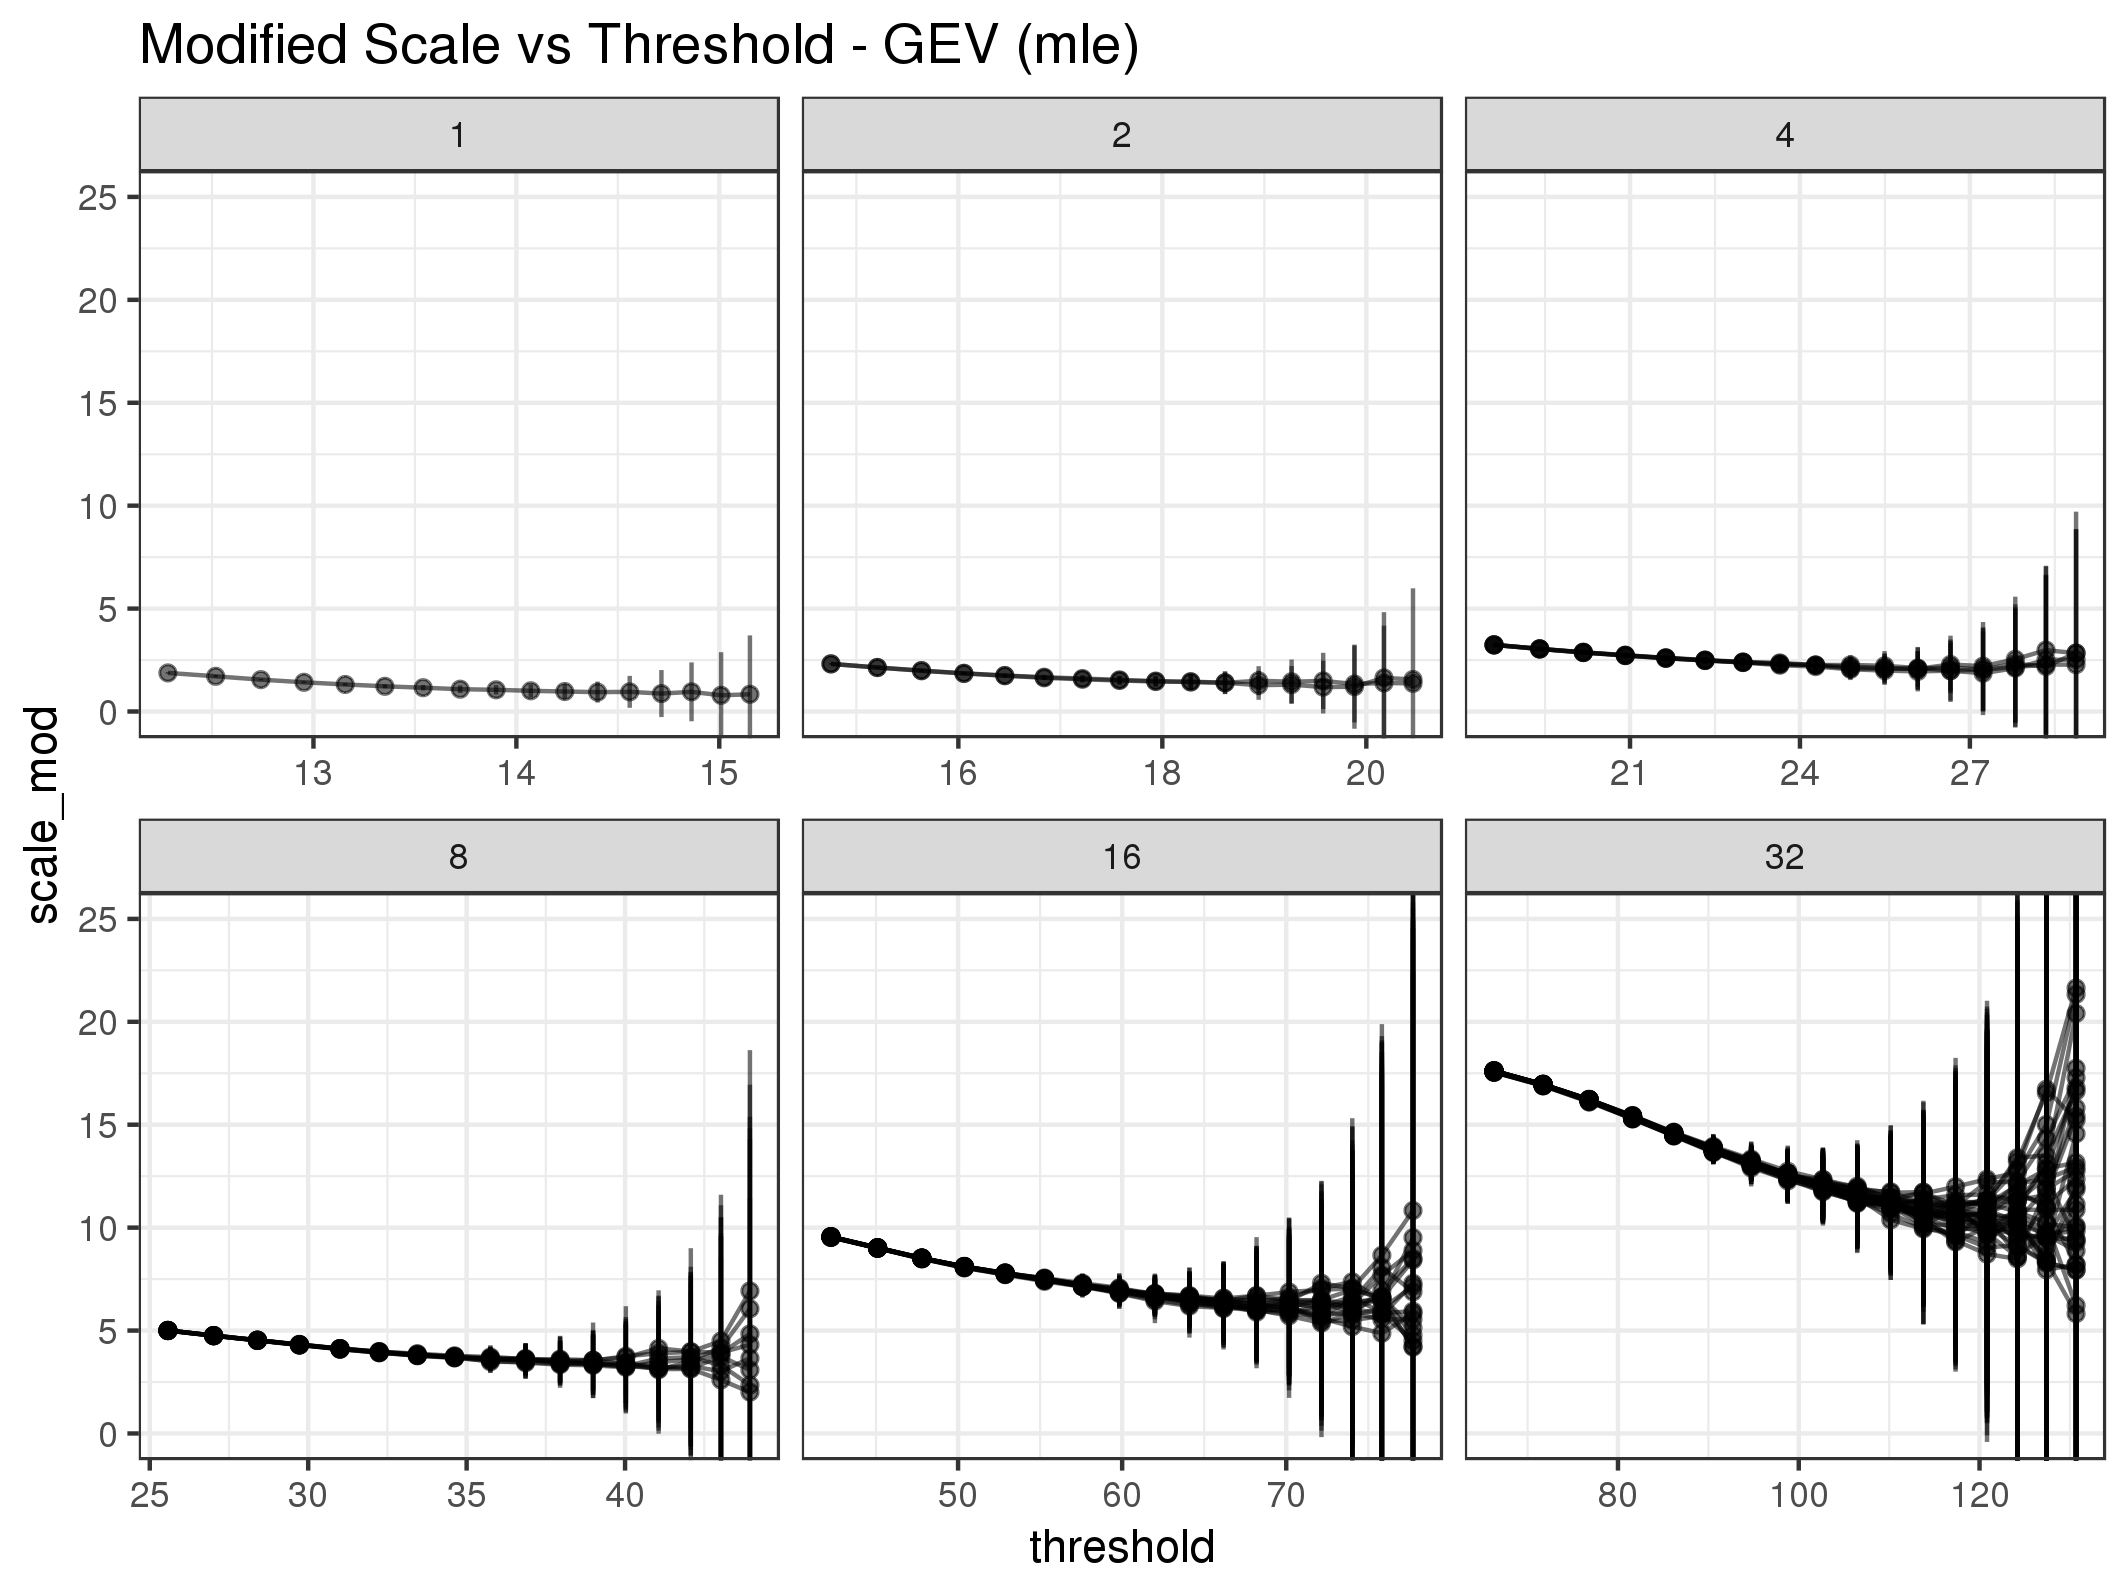
\includegraphics[width=\linewidth]{fig/modscale_gev_mle_RK401_1e7_maxt05_1e7.png}
	\caption{Ensemble average of \textit{modified scale} parameter over 92 simulations. Each cluster is treated separately.}
	\label{fig:modscale_mle}
\end{figure}

\subsubsection{Method of Moments}
Results are shown in Fig. \ref{fig:shape_mom} and \ref{fig:modscale_mom}.
\\Script:
\begin{itemize}
	\item moments computation: \href{https://github.com/marco-cucchi/L96gev/commit/240d6d0471ddc3fc53789e43e03a87013d032b86#diff-9576f7ab149830e9a08339b0fc9f2569}{240d6d0}
	\item parameters derivation and plots: \href{https://github.com/marco-cucchi/L96gev/commit/97925ef80db61ade1851bb7c41948d7f13f3b91f#diff-503bcadc356f924b6a536c1b0796b054}{97925ef}
\end{itemize}

\begin{figure}
	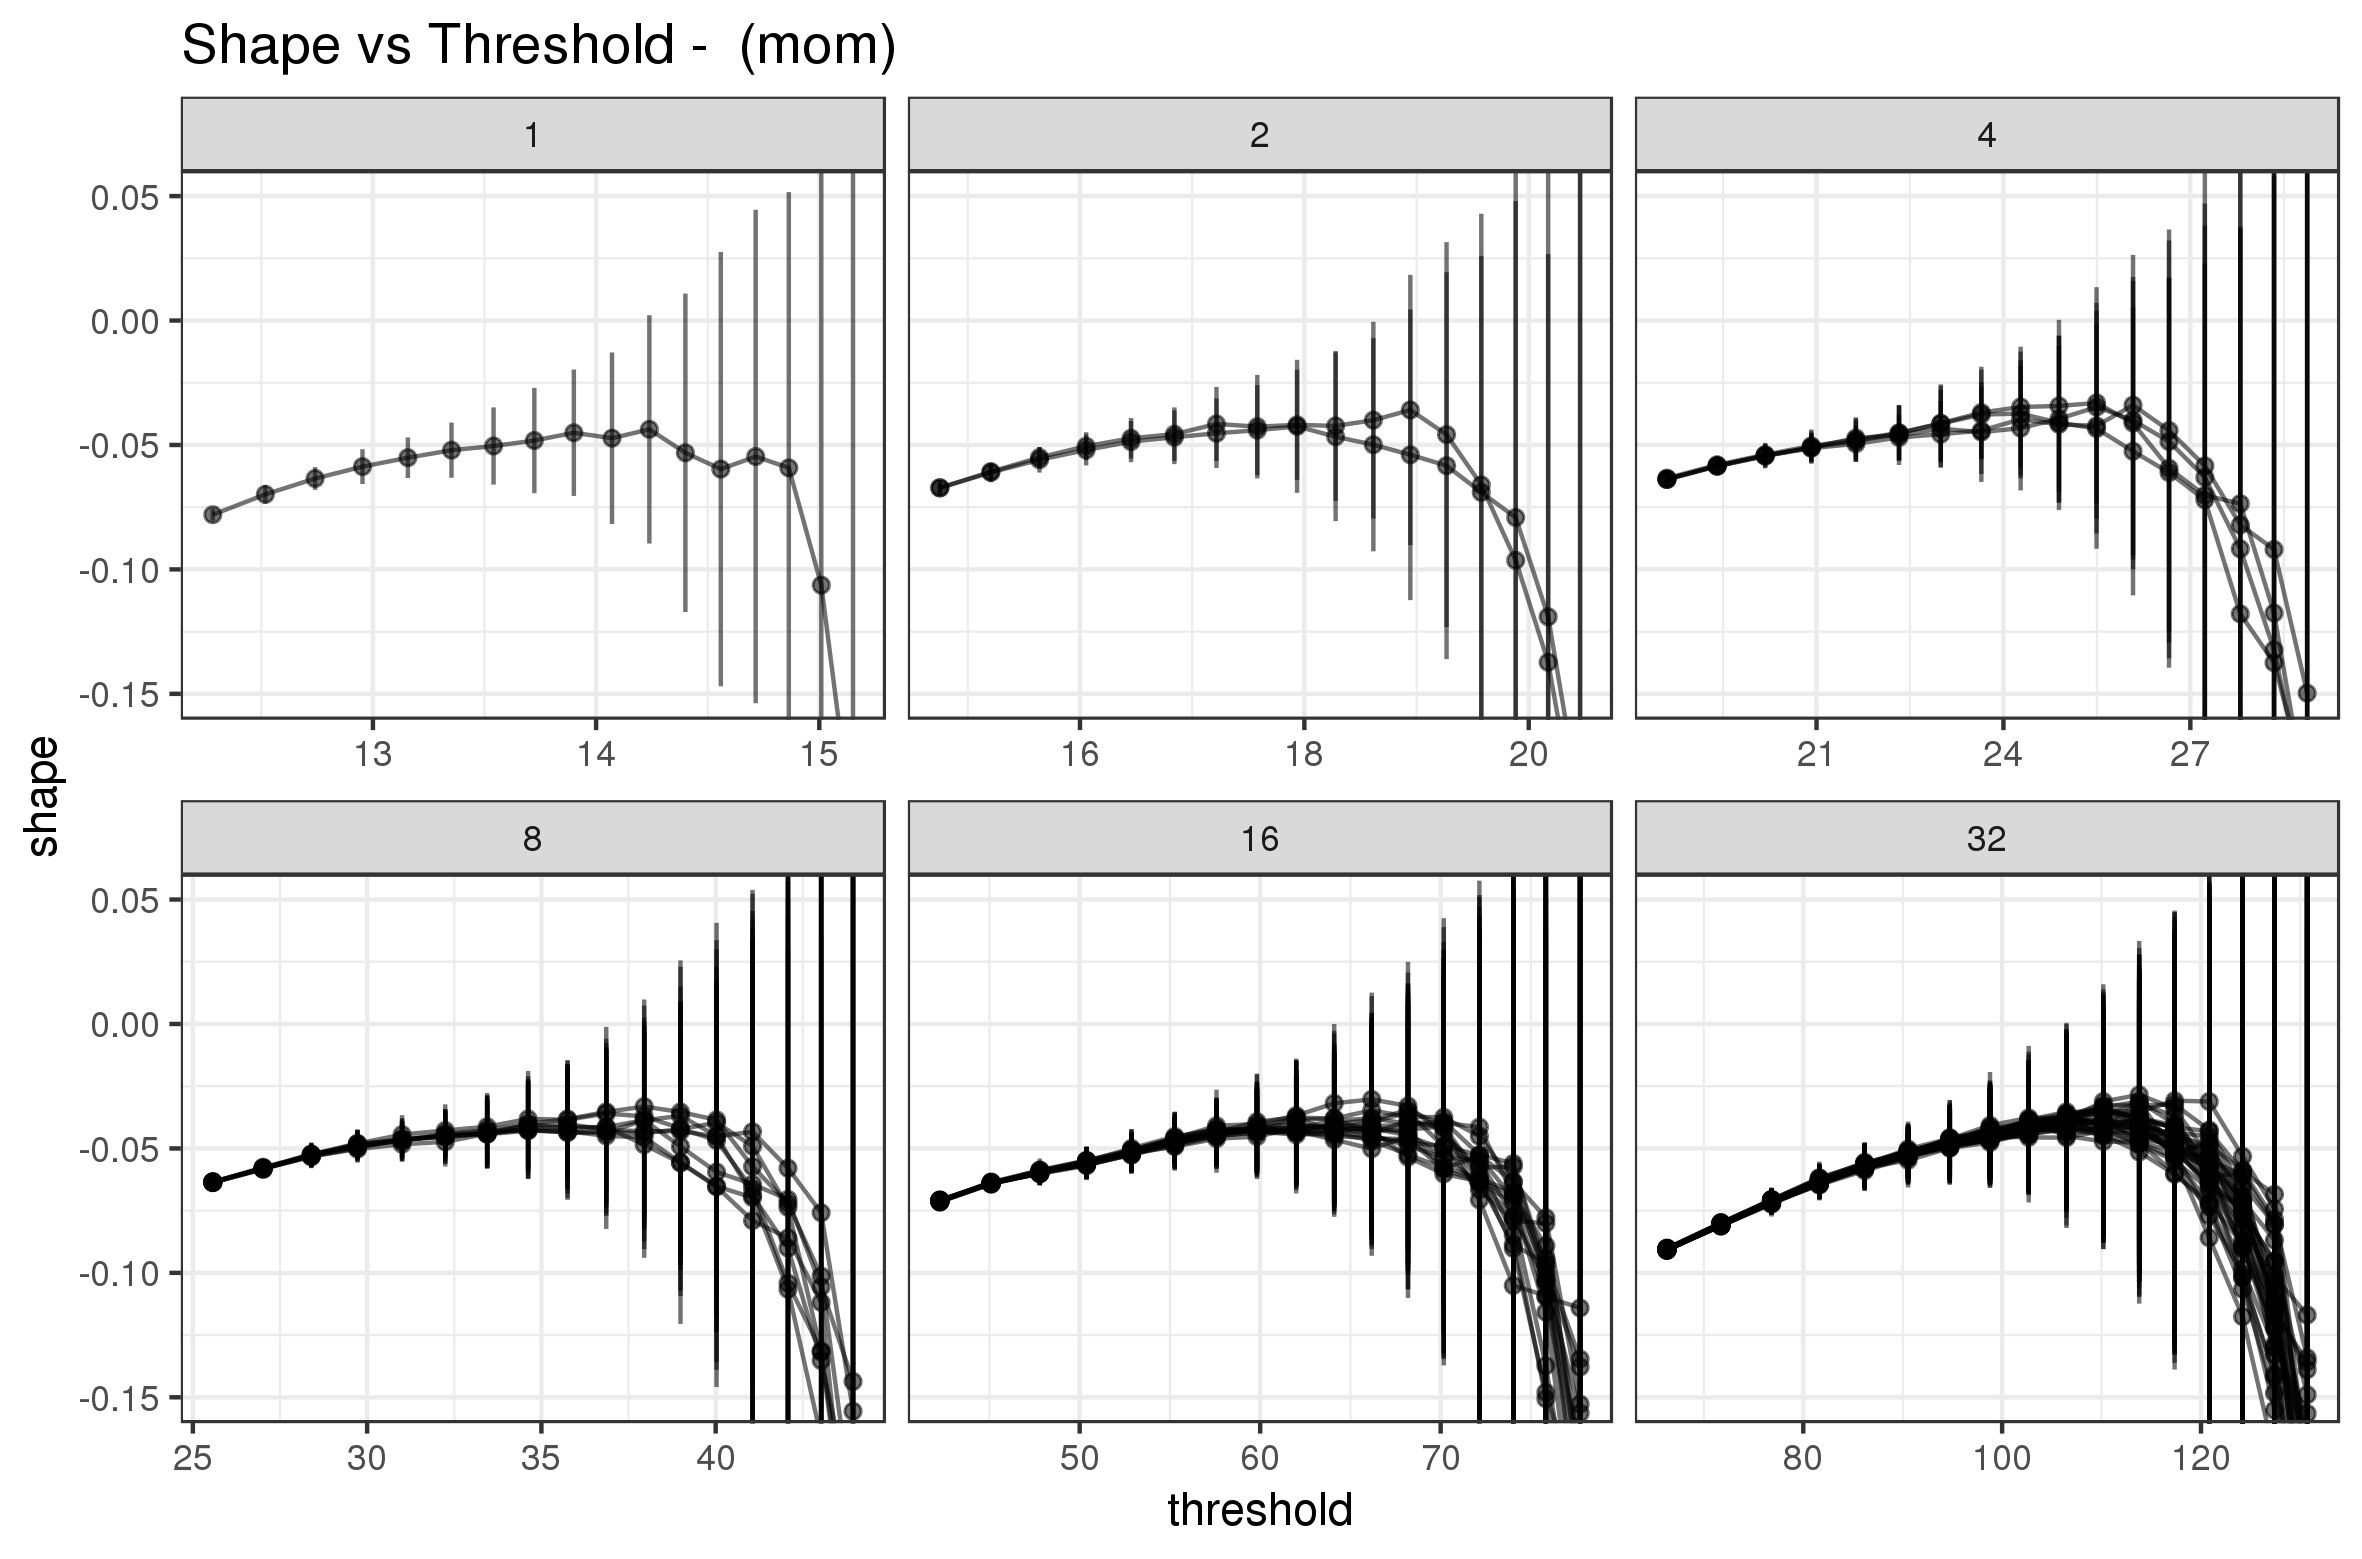
\includegraphics[width=\linewidth]{fig/shape_mom_RK401_1e7_maxt05_1e7.png}
	\caption{Ensemble average of \textit{shape} parameter over 92 simulations. Each cluster is treated separately.}
	\label{fig:shape_mom}
\end{figure}

\begin{figure}
	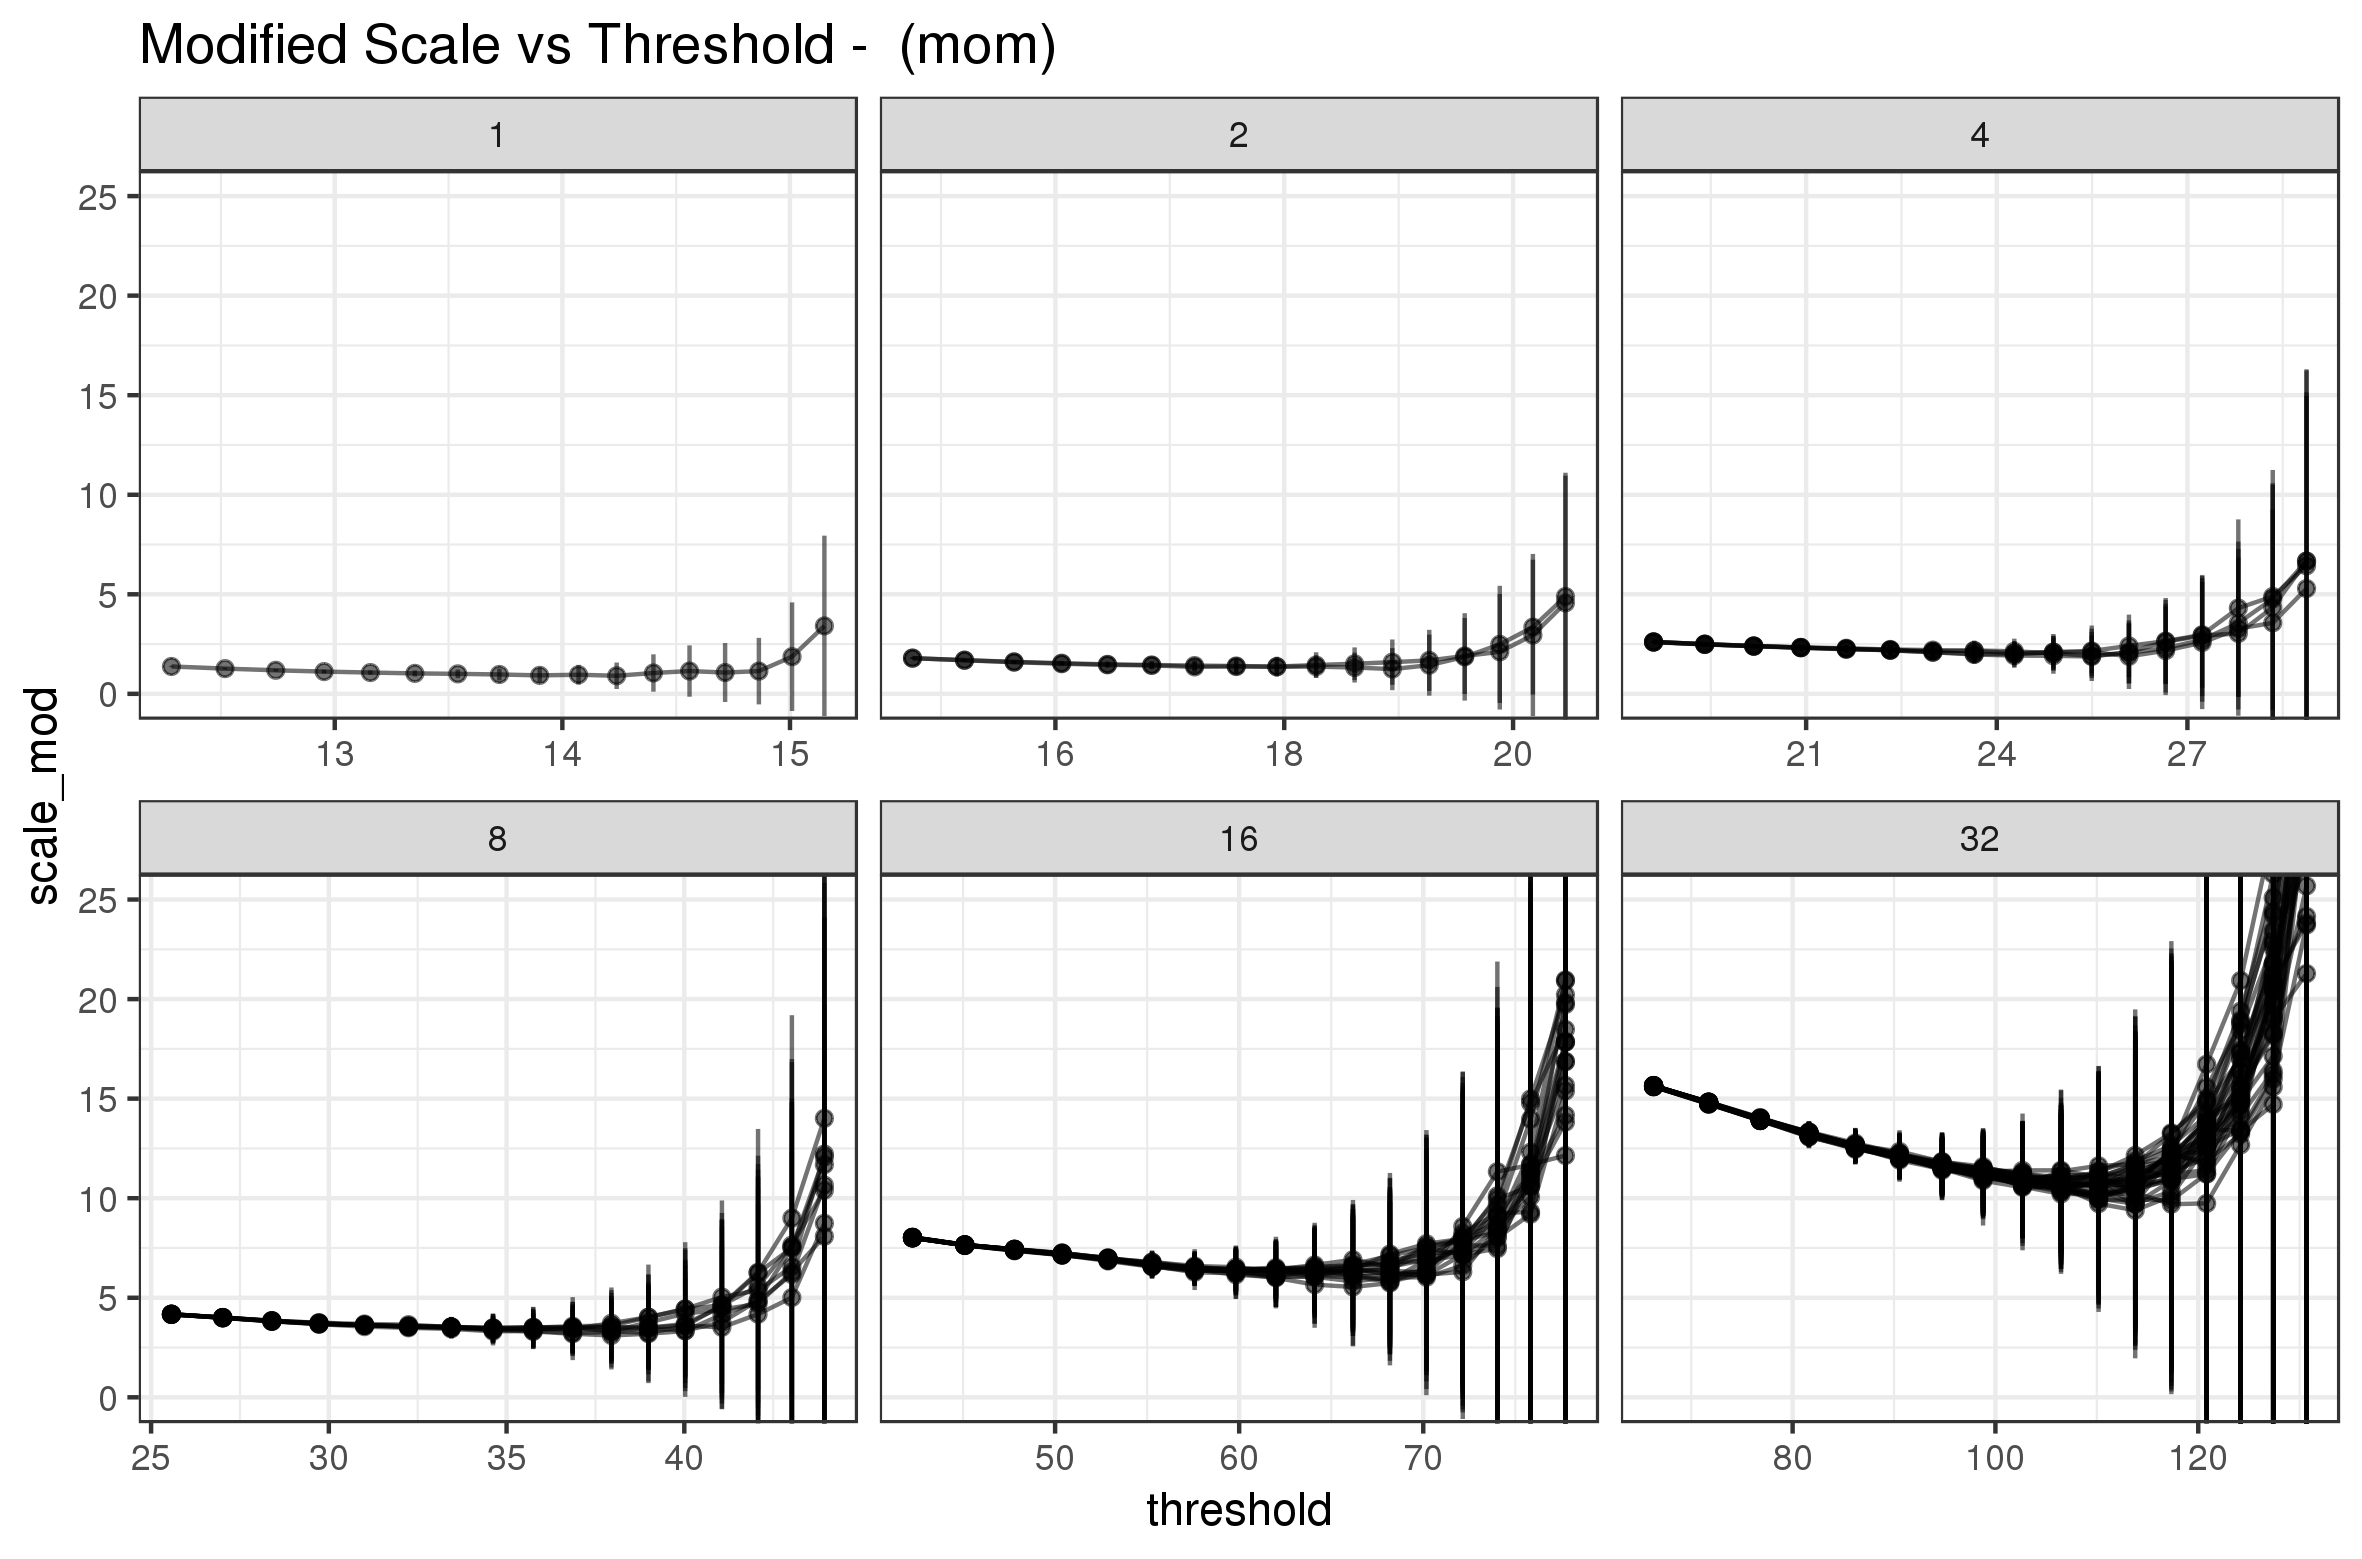
\includegraphics[width=\linewidth]{fig/modscale_mom_RK401_1e7_maxt05_1e7.png}
	\caption{Ensemble average of \textit{modified scale} parameter over 92 simulations. Each cluster is treated separately.}
	\label{fig:modscale_mom}
\end{figure}

\section{LRT and the Lorenz-96 model}

We aim to apply Ruelle response theory \cite{Ruelle}\cite{Bodai} to predict the response of different observables to the action of both constant and time-dependent forcings to our Lorenz-96 model.
Among these observables, we will focus our efforts on ones describing statistics of extreme events.

\subsection{Background}

Given a \textit{nonautonomous dissipative dynamical system} in the form
\begin{equation}
\dot{x}=F(x)+\epsilon g(x) f(t)
\end{equation}
and a scalar observable $\Psi(x)$, Ruelle's response theory \cite{Ruelle} asserts that its mean $\langle\Psi\rangle=\int \mu_{t}(d x) \Psi(x)$ can be decomposed as
\begin{equation}
\langle\Psi\rangle(t)=\sum_{j=1}^{\infty} \epsilon^{j}\langle\Psi\rangle^{(j)} +\langle\Psi\rangle_{0}
\end{equation}
where the $\langle\Psi\rangle$ can be expressed as multiple convolution integrals involving the pertinent Green's functions \cite{LucariniClimateChange}. In the linear (first-order) approximation, we can thus express the response to the forcing $f(t)$ as
\begin{equation}
\Delta\langle\Psi\rangle(t)=\langle\Psi\rangle^{(1)}(t)=G_{\Psi}^{(1)}(t) * f(t)=\int_{-\infty}^{\infty} d \tau G_{\Psi}^{(1)}(\tau) f(t-\tau)
\end{equation}
where the Green's function has been established by Ruelle to take the form of
\begin{equation}
G_{\Psi}^{(1)}(t)=\int d x \Psi(x)\left(\exp \left[t L_{f}\right]\left[L_{g} \overline{\mu}\right]\right)(x)
\end{equation}
where $\overline{\mu}(d x)$ is the natural invariant measure/probability distribution of the autonomous system $(f = 0)$, and operators are defined as $L_{f} \mu=-\operatorname{div}(f \mu)$ and $L_{g} \mu=-\operatorname{div}(g \mu)$, in the notation of \cite{Abramov}.

Following \cite{Bodai}, in a discrete-time scenario sample values of the response with the sampling $\Psi[n]=\Psi(t=(n+\nu) T)$ at any phase $\nu \in[0,1]$ obey:

\begin{equation}
\langle\hat{\Psi}\rangle^{(1)}[n]=\sum_{k=-\infty}^{\infty} h_{\Psi}[k] f[n-k]=h_{\Psi}[n] * f[n]
\end{equation}
where the discrete-time (DT) impulse response or DT Green's function $h_{\Psi}[n]$ is the response $\langle\hat{\Psi}_{\perp}\rangle$ to a Kronecker delta function forcing: $f[n]=\delta[n]=1$ if $n=0$ and 0 otherwise. Unlike the Dirac delta \footnote{Never mentioned before.\label{fn8}}, the Kronecker delta can be realised for numerical purposes. It is equivalent to applying a step forcing and taking the difference: 

\begin{equation} \label{eq:differencing}
h_{\Psi}[n]=\langle\hat{\Psi}_{\Gamma}\rangle[n]-\langle\hat{\Psi}_{\Gamma}\rangle[n-1]
\end{equation}
In the case of a \textit{finite} time-series, $f[l]$ and $h_{\Psi}[l]$, $l=0, \dots, L-1$, the response $h_{\Psi} * f[l], l=0, \dots, L-1$ can be computed as:

\begin{equation}
\left(h * f_{N}\right)[n=0, \ldots, N-1]=\sum_{k=0}^{N-1} h[k] f_{N}[n-k]=\mathrm{DFT}^{-1}\{\mathrm{DFT}\{h\} \mathrm{DFT}\{f\}\},
\end{equation}
where DFT is the discrete Fourier transform.

\subsection{The Experiment}

We want to make predictions on the average response of observables of the Lorenz-96 system to different forcings.

We use as identification forcing \footnote{Never mentioned before. See Par. 2.2 in \cite{Bodai}.\label{fn9}} a \textit{step forcing of unit intensity}, activated at time $t_0=0$. An ensemble of 10000 simulations of length $T=100$ is generated \footnote{Describe more how simulations are generated} with this forcing and for the system at rest ($F=8$), and responses for the different observables are averaged among ensemble members.

The same procedure is repeated using as identification forcing a \textit{step forcing of negative unit intensity}. The semi-difference of the two average responses is then used to compute the DT Green's function $h_{\Psi}[n]$ as described in \eqref{eq:differencing} \footnote{This procedure less noisy (and more accurate?) results. \textbf{Ask Valerio for reference}.}

Results are compared with the ones obtained using only response to the (positive) unit step forcing to compute response function.

For each simulation, only one node is considered.
 
Two observables are taken into considerations:

\begin{itemize}
	\item Energy
	\item Above threshold (between thresholds) occurrence of energy values
\end{itemize}

\subsubsection{Energy}

Energy is computed at single locations, as

\begin{equation}
e_n=\frac{1}{2} x_n^{2}
\end{equation}

\subsubsection{Above threshold occurrence of energy values}

Starting from energy values $e_n$, this observable $o_{n, e_t}$ is computed as

\begin{equation}
o_{n, t}=H[e_n - e_t],
\end{equation}
where $H$ is the Heaviside step function

\begin{equation}
	H[x]=\left\{\begin{array}{ll}{0,} & {x<0} \\ {1,} & {x \geq 0}\end{array}\right.
\end{equation}
and $e_t$ is some energy value.

Once averaged over ensemble members, this observable yields the average frequency of energy values above a certain threshold. Using as thresholds $e_t$ high quantiles of the energy distribution for the system at rest, if LRT works we could use it to predict changes in the frequency of extreme (above high thresholds) events.

More generally, we can look at \textbf{between-thresholds occurrence}, computed as

\begin{equation}
o_{n, t_1, t_2}=H[e_n - e_{t_1}] - H[e_n - e_{t_2}],
\end{equation}
with $e_{t_1} < e_{t_2}$. Again, averaging this observable over ensemble members yields the average frequency of energy values between the two thresholds $e_{t_1}$ and $e_{t_2}$. Using LRT, \textbf{we could thus theoretically predict changes in the shape of energy values probability distribution}.

\subsection{Results}\label{results}

In this section, comparisons between actual and predicted (via LRT) responses are shown for \textbf{above} and \textbf{below-thresholds occurrences} observables.
As thresholds, energy percentiles (computed on the system at rest) have been taken (see Figures' titles).
The following forcings have been considered:

\begin{itemize}
	\item \textbf{Step forcing}
		\begin{equation}
		F[t]=\left\{\begin{array}{ll}{8,} & {t \leq 0} \\ {11,} & {t > 0}\end{array}\right.
		\end{equation}		
	\item \textbf{Linearly increasing forcing}
		\begin{equation}
		F[t]=\left\{\begin{array}{ll}{F_0 + C t,} & {t \leq t_f} \\ {F_0 + C t_f,} & {t > t_f}\end{array}\right.
		\end{equation}
		with two sets of parameters $(F_0, C, t_f)$, namely $(8, 0.03, 100)$ and $(8, 0.3, 10)$.
\end{itemize}
Results are shown in Figures \ref{fig:pred_bin_S_30}, \ref{fig:pred_bin_L_003_100} and \ref{fig:pred_bin_L_03_10}.

\begin{figure}[!htb]
	\centering
	\textbf{Step Forcing - $\Delta F=3$}\par\medskip
	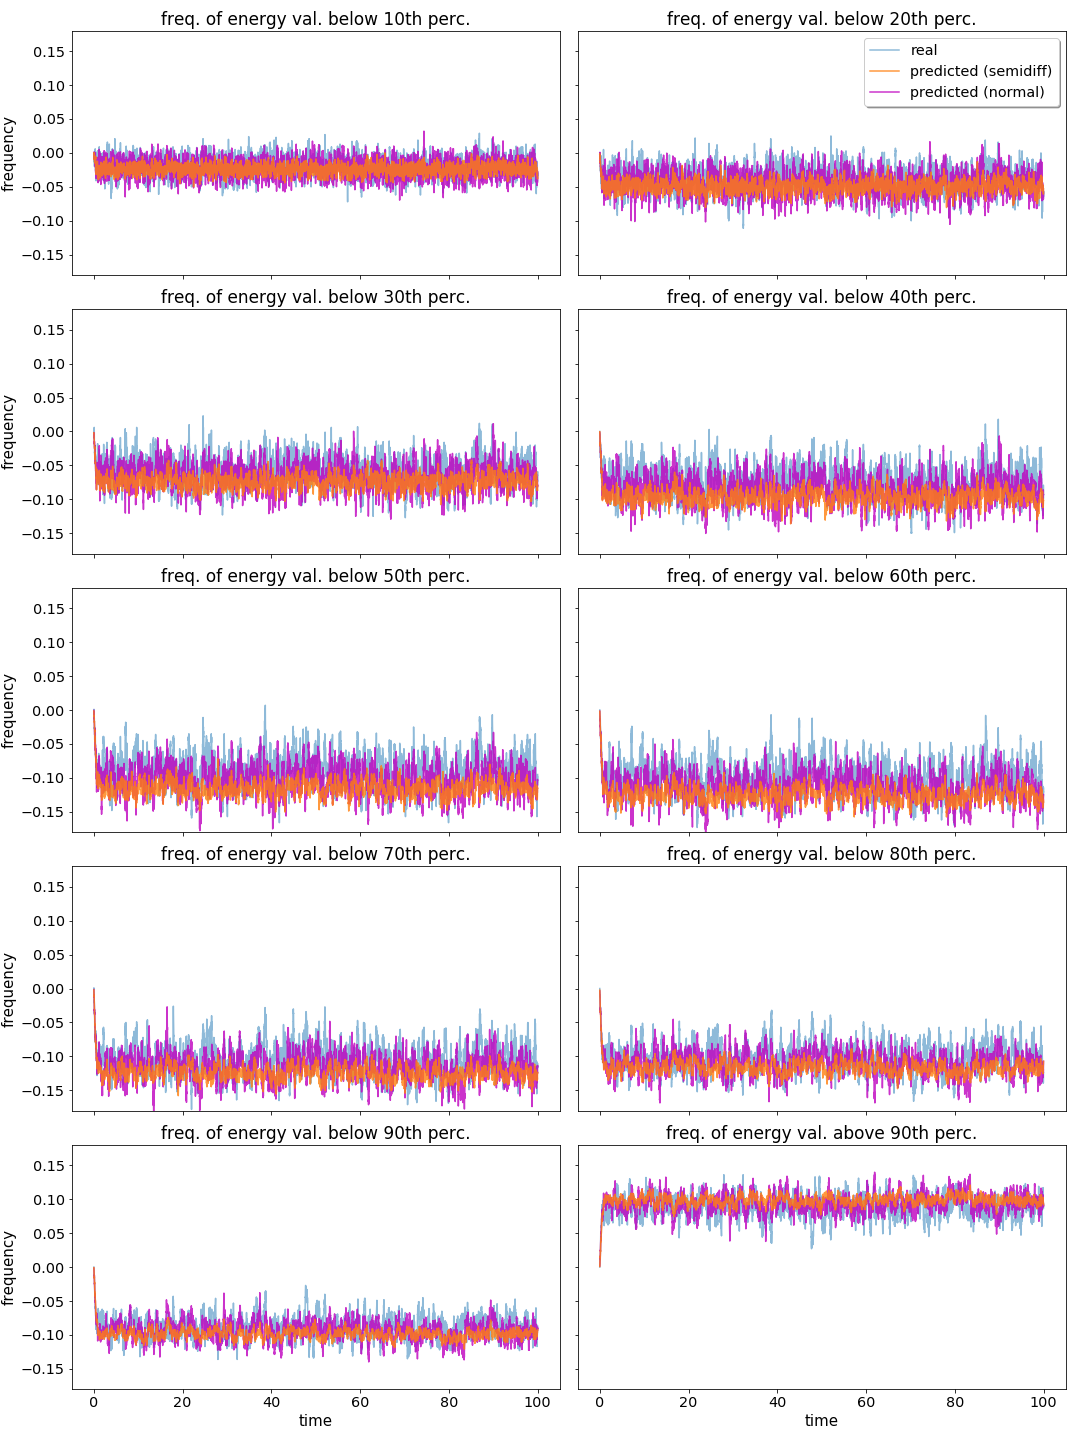
\includegraphics[width=0.9\linewidth]{fig/pred_below_S_30.png}
	\caption{Real vs. predicted average responses of \textbf{occurrence observables} for \textbf{step forcing}, activated at time $t=0$ with intensity $\Delta F = 3$.}
	\label{fig:pred_bin_S_30}
\end{figure}

\begin{figure}[!h]
	\centering
	\textbf{Linear Forcing - $(F_0=8, C=0.03, t_f=100)$}\par\medskip
	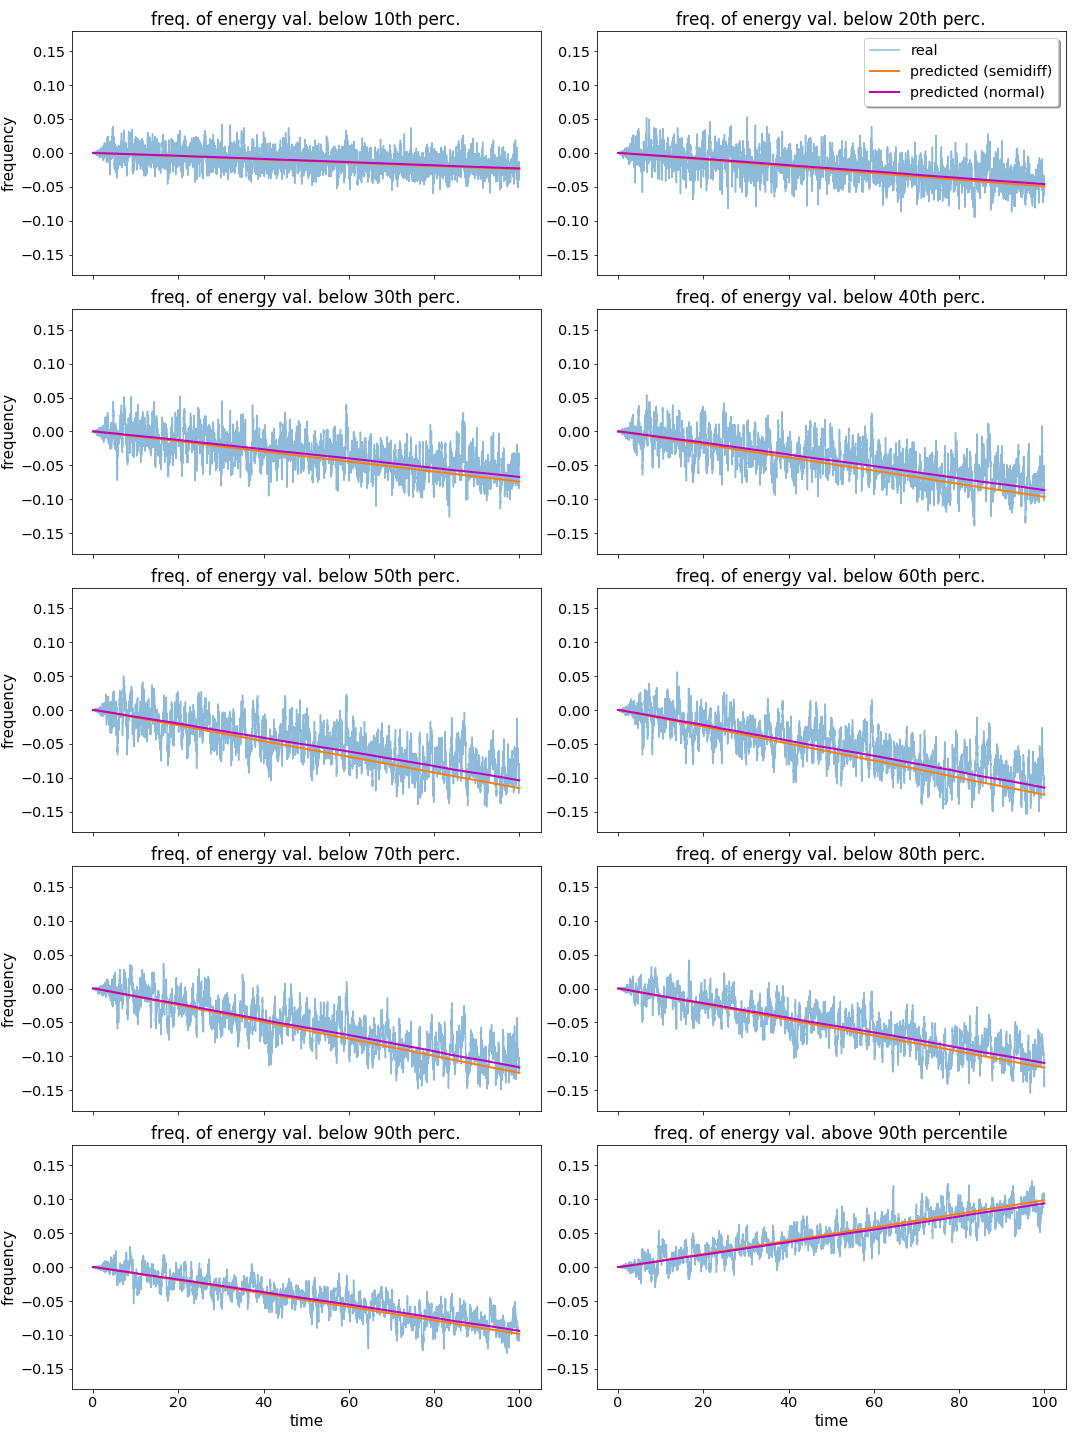
\includegraphics[width=0.9\linewidth]{fig/pred_below_L_003_100.png}
	\caption{Real vs. predicted average responses of \textbf{occurrence observables} for \textbf{linear forcing}, activated at time $t_i=0$, deactivated at time $t_f=100$, with linear coefficient $C=0.03$.}
	\label{fig:pred_bin_L_003_100}
\end{figure}

\begin{figure}[!h]
	\centering
	\textbf{Linear Forcing - $(F_0=8, C=0.3, t_f=10)$}\par\medskip
	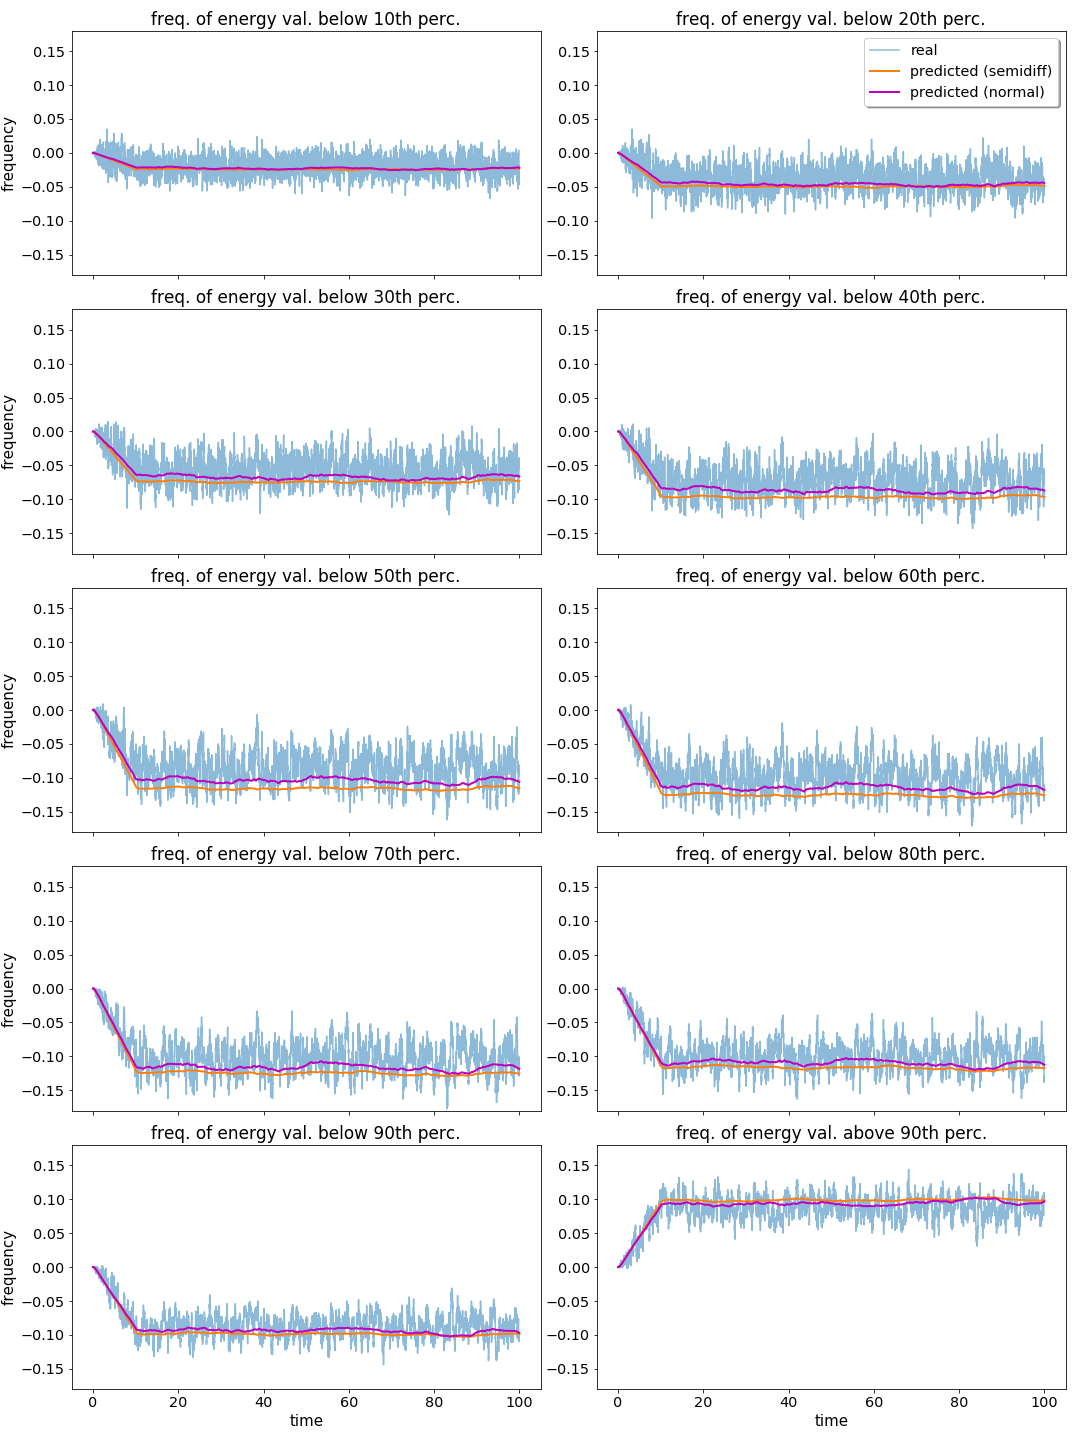
\includegraphics[width=0.9\linewidth]{fig/pred_below_L_03_10.png}
	\caption{Real vs. predicted average responses of \textbf{occurrence observables} for \textbf{linear forcing}, activated at time $t_i=0$, deactivated at time $t_f=10$, with linear coefficient $C=0.3$.}
	\label{fig:pred_bin_L_03_10}
\end{figure}

\subsubsection{Comments}

Why predicted responses in linear forcing cases are so much less noisy than in the step forcing case?

\newpage

\subsection{A closer look at higher percentiles}

In Figure \ref{fig:pred_energy_exceed_099q} results are shown for the same forcings explored in \ref{results}, but for frequency of values below and above a higher percentile ($99^{th}$). 

From the plots \textit{a discrepancy is evident between observations and predictions}, which was not so obvious for larger percentiles' intervals. Furthermore, \textit{the discrepancy is bigger} (especially for exceedances of $99^{th}$ percentile) \textit{when using semi-difference of responses for computing response function}.

The discrepancy could be due to the fact that \textit{the applied forcings are too strong for the linear approximation to be valid}. In order to explore this, Fig. \ref{fig:pred_energy_exceed_099q_L} shows predictions for exceedances of the $99^{th}$ percentile for the following forcings:

\begin{itemize}
	\item Linear Forcing - $F_0=8, C=0.03, t_f=100$
	\item Linear Forcing - $F_0=8, C=0.02, t_f=100$
	\item Linear Forcing - $F_0=8, C=0.01, t_f=100$
	\item Linear Forcing - $F_0=8, C=0.3, t_f=10$
	\item Linear Forcing - $F_0=8, C=0.2, t_f=10$
	\item Linear Forcing - $F_0=8, C=0.1, t_f=10$
\end{itemize}

From Fig. \ref{fig:pred_energy_exceed_099q_L}, it is clear how \textbf{things get better lowering the forcing intensity}, and again it is confirmed the \textbf{higher accuracy of predictions made using only the unit step forcing to derive response function}.

As a consequence, for the moment, \textbf{predictions will be made against forcings having up to $\Delta F=2$ as maximum intensity, and deriving response functions using only unit step forcing}. 

\begin{figure}[!ht]
	\centering
	\begin{subfigure}[b]{0.48\textwidth}
		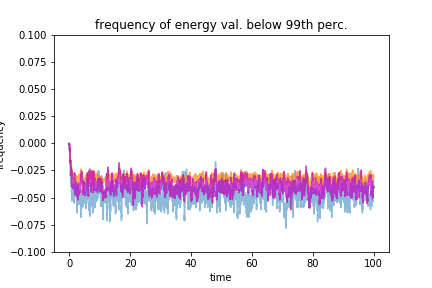
\includegraphics[width=1\linewidth]{fig/pred_energy_bin_00q_099q_S_30.png}
		\caption{Step forcing, $\Delta F=3$}
		\label{fig:pred_energy_bin_00q_099q_S_30}
	\end{subfigure}%
	\begin{subfigure}[b]{0.48\textwidth}
		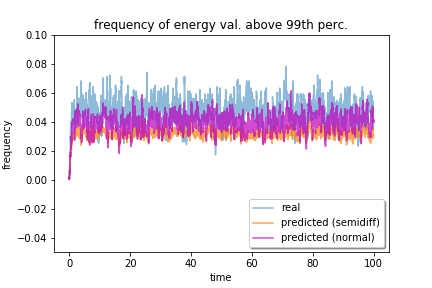
\includegraphics[width=1\linewidth]{fig/pred_energy_exceed_099q_S_30.png}
		\caption{Step forcing, $\Delta F=3$}
		\label{fig:pred_energy_exceed_099q_S_30}
	\end{subfigure}
	\begin{subfigure}[b]{0.48\textwidth}
		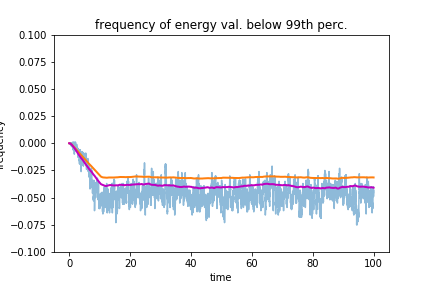
\includegraphics[width=1\linewidth]{fig/pred_energy_bin_00q_099q_L_03_10.png}
		\caption{Linear Forcing - $(F_0=8, C=0.3, t_f=10)$}
		\label{fig:pred_energy_bin_00q_099q_L_03_10}
	\end{subfigure}%
	\begin{subfigure}[b]{0.48\textwidth}
		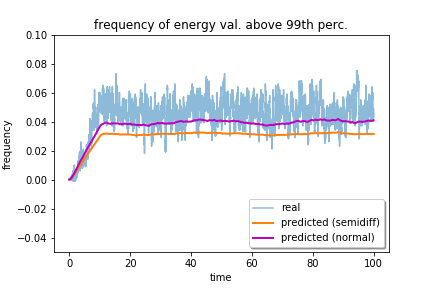
\includegraphics[width=1\linewidth]{fig/pred_energy_exceed_099q_L_03_10.png}
		\caption{Linear Forcing - $(F_0=8, C=0.3, t_f=10)$}
		\label{fig:pred_energy_exceed_099q_L_03_10}
	\end{subfigure}
	\begin{subfigure}[b]{0.48\textwidth}
		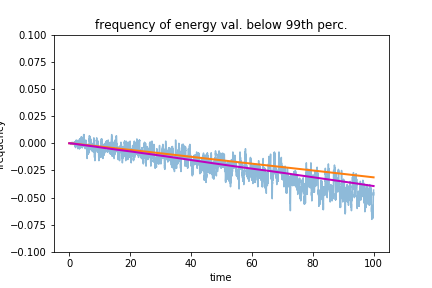
\includegraphics[width=1\linewidth]{fig/pred_energy_bin_00q_099q_L_003_100.png}
		\caption{Linear Forcing - $(F_0=8, C=0.03, t_f=100)$}
		\label{fig:pred_energy_bin_00q_099q_L_003_100}
	\end{subfigure}%
	\begin{subfigure}[b]{0.48\textwidth}
		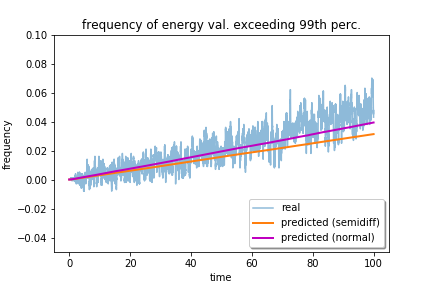
\includegraphics[width=1\linewidth]{fig/pred_energy_exceed_099q_L_003_100.png}
		\caption{Linear Forcing - $(F_0=8, C=0.03, t_f=100)$}
		\label{fig:pred_energy_exceed_099q_L_003_100}
	\end{subfigure}
	\caption{predictions for exceedance of $99^{th}$ percentile and occurrence between $98^{th}$ and $99^{th}$ percentiles}
	\label{fig:pred_energy_exceed_099q}
\end{figure}

\begin{figure}[!ht]
	\centering
	\begin{subfigure}[b]{0.48\textwidth}
		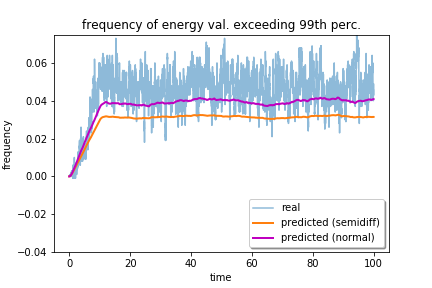
\includegraphics[width=1\linewidth]{fig/pred_energy_exceed_099q_L_03_10_2.png}
		\caption{Linear Forcing - $(F_0=8, C=0.3, t_f=10)$}
		\label{fig:pred_energy_exceed_099q_L_03_10_comp}
	\end{subfigure}%
	\begin{subfigure}[b]{0.48\textwidth}
		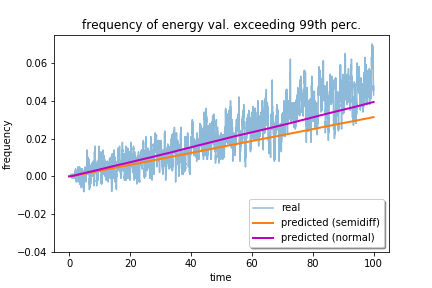
\includegraphics[width=1\linewidth]{fig/pred_energy_exceed_099q_L_003_100_2.png}
		\caption{Linear Forcing - $(F_0=8, C=0.03, t_f=100)$}
		\label{fig:pred_energy_exceed_099q_L_003_100_comp}
	\end{subfigure}
	\begin{subfigure}[b]{0.48\textwidth}
		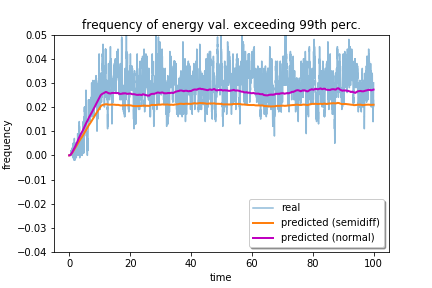
\includegraphics[width=1\linewidth]{fig/pred_energy_exceed_099q_L_02_10.png}
		\caption{Linear Forcing - $(F_0=8, C=0.2, t_f=10)$}
		\label{fig:pred_energy_exceed_099q_L_02_10_comp}
	\end{subfigure}%
	\begin{subfigure}[b]{0.48\textwidth}
		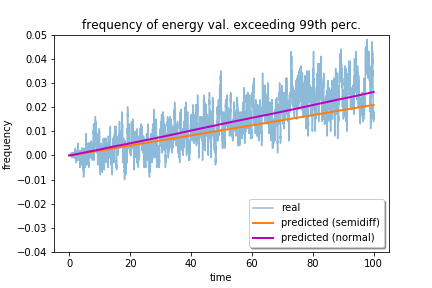
\includegraphics[width=1\linewidth]{fig/pred_energy_exceed_099q_L_002_100.png}
		\caption{Linear Forcing - $(F_0=8, C=0.02, t_f=10)$}
		\label{fig:pred_energy_exceed_099q_L_002_100_comp}
	\end{subfigure}
	\begin{subfigure}[b]{0.48\textwidth}
		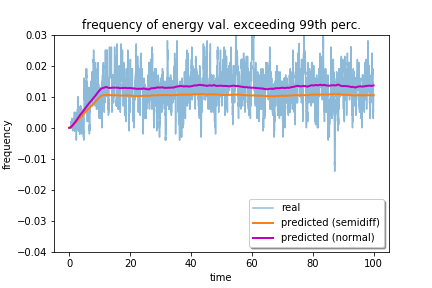
\includegraphics[width=1\linewidth]{fig/pred_energy_exceed_099q_L_01_10.png}
		\caption{Linear Forcing - $(F_0=8, C=0.1, t_f=100)$}
		\label{fig:pred_energy_exceed_099q_L_01_10_comp}
	\end{subfigure}%
	\begin{subfigure}[b]{0.48\textwidth}
		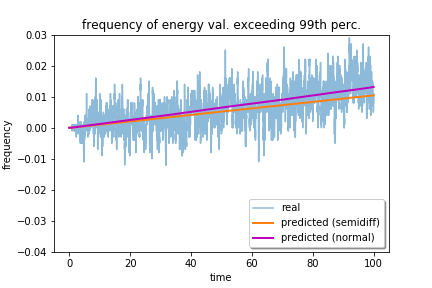
\includegraphics[width=1\linewidth]{fig/pred_energy_exceed_099q_L_001_100.png}
		\caption{Linear Forcing - $(F_0=8, C=0.01, t_f=100)$}
		\label{fig:pred_energy_exceed_099q_L_001_100_comp}
	\end{subfigure}
	\caption{predictions for exceedance of $99^{th}$ percentile for different linear forcings}
	\label{fig:pred_energy_exceed_099q_L}
\end{figure}

\clearpage

\subsection{Prediction of changes in Energy values distribution}

In this section predictions of changes in the Energy values distribution are shown for the following forcings:

\begin{itemize}
	\item Linear Forcing - $F_0=8, C=0.01, t_f=100$
	\item Linear Forcing - $F_0=8, C=0.02, t_f=100$
\end{itemize}
The plots are produced as follows:
\begin{itemize}
	\item \textbf{CDF} 
	
	on the $x$ axis, percentiles from the $1^{st}$ to the $100^{th}$ as computed from the \textit{unperturbed} system are reported; on the $y$ axis, frequency of observations below corresponding percentile in the \textit{unperturbed} and \textit{perturbed} (at $t=50$ and $t=100$) are reported.
	  
	\item \textbf{PDF}
	
	starting from arrays of values \textbf{x} and \textbf{y} used for CDF, \textbf{x'} and \textbf{y'} are computed as:
	
	\begin{itemize}
		\item $x'_i = x_i + \frac{x_{i+1} - x_i}{2}$
		\item $y'_i = \frac{y_{i+1} - y_i}{x_{i+1} - x_i}$
	\end{itemize}
	
	
\end{itemize}

\begin{figure}[!ht]
	\centering
	\begin{subfigure}[b]{0.48\textwidth}
		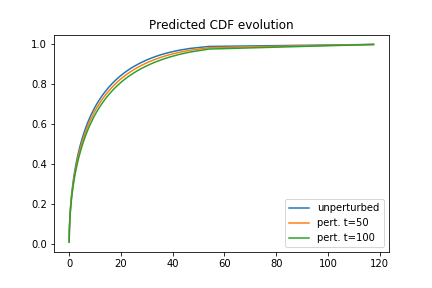
\includegraphics[width=1\linewidth]{fig/pred_cdf_energy_L_001_100.png}
		\caption{Step forcing, $\Delta F=3$}
		\label{fig:pred_cdf_energy_L_001_100}
	\end{subfigure}%
	\begin{subfigure}[b]{0.48\textwidth}
		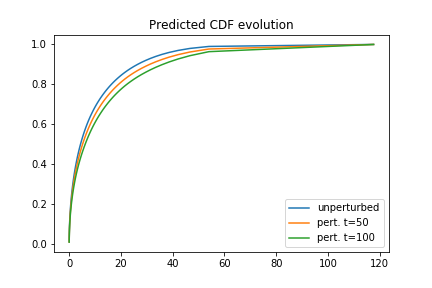
\includegraphics[width=1\linewidth]{fig/pred_cdf_energy_L_002_100.png}
		\caption{Step forcing, $\Delta F=3$}
		\label{fig:pred_cdf_energy_L_002_100}
	\end{subfigure}
	\begin{subfigure}[b]{0.48\textwidth}
		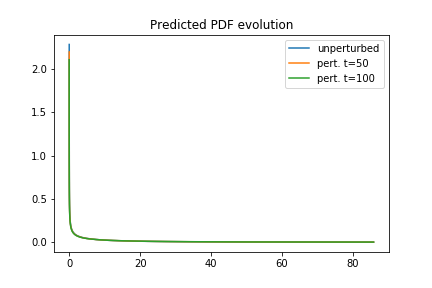
\includegraphics[width=1\linewidth]{fig/pred_pdf_energy_L_001_100.png}
		\caption{Linear Forcing - $(F_0=8, C=0.3, t_f=10)$}
		\label{fig:pred_pdf_energy_L_001_100}
	\end{subfigure}%
	\begin{subfigure}[b]{0.48\textwidth}
		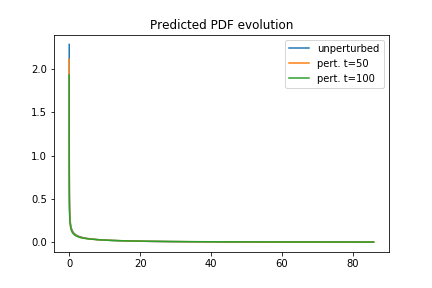
\includegraphics[width=1\linewidth]{fig/pred_pdf_energy_L_002_100.png}
		\caption{Linear Forcing - $(F_0=8, C=0.3, t_f=10)$}
		\label{fig:pred_pdf_energy_L_002_100}
	\end{subfigure}
	\begin{subfigure}[b]{0.48\textwidth}
		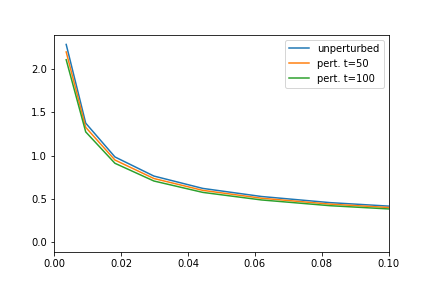
\includegraphics[width=1\linewidth]{fig/pred_pdf_zoom_energy_L_001_100.png}
		\caption{Linear Forcing - $(F_0=8, C=0.03, t_f=100)$}
		\label{fig:pred_pdf_zoom_energy_L_001_100}
	\end{subfigure}%
	\begin{subfigure}[b]{0.48\textwidth}
		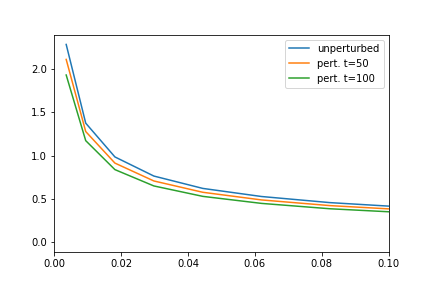
\includegraphics[width=1\linewidth]{fig/pred_pdf_zoom_energy_L_002_100.png}
		\caption{Linear Forcing - $(F_0=8, C=0.03, t_f=100)$}
		\label{fig:pred_pdf_zoom_energy_L_002_100}
	\end{subfigure}
	\caption{predictions for exceedance of $99^{th}$ percentile and occurrence between $98^{th}$ and $99^{th}$ percentiles}
	\label{fig:pred_energy_cdf_pdf}
\end{figure}


\clearpage

\bibliography{bibliography}
\bibliographystyle{ieeetr}

\end{document}